% !TeX program = xelatex
% !TeX encoding = UTF-8
\documentclass[12pt,a4paper]{article}

\usepackage[margin=2.5cm]{geometry}
\usepackage{amsmath,amssymb,amsthm}
\usepackage{xeCJK}
\setCJKmainfont{Microsoft JhengHei}
\usepackage{graphicx}

\usepackage[hidelinks]{hyperref}
\usepackage{fancyhdr}

% Total physical pages recorded by LaTeX; compile twice after page-count changes.
\makeatletter
\newcommand{\totalpages}{\@abspage@last}
\makeatother
\pagestyle{fancy}
\fancyhf{}
\renewcommand{\headrulewidth}{0pt}
\fancyfoot[C]{\thepage/\totalpages}
% The title page uses the plain page style.
\fancypagestyle{plain}{%
  \fancyhf{}%
  \renewcommand{\headrulewidth}{0pt}%
  \fancyfoot[C]{\thepage/\totalpages}%
}

\title{Linear System --- Homework 1}
\author{姓名：葉彥辰\quad 學號：P46154345}
\date{}

\begin{document}
\maketitle

\section*{Exercise 1}
Consider a system described by a single $n$th-order linear differential equation of
the form
\[
q^{(n)} + a_{n-1}q^{(n -1)} + \dots + a_1\dot q + a_0q = u
\]
where $q(t)\in\mathbb{R}$ and $q^{(n)}:=\dfrac{d^nq}{dt^n}$.
By appropriate definition of state variables, obtain a first order state space
description of this system.

\subsection*{Solution}

Define the state variables first
\begin{equation*}
	x_1 = q,\quad x_2 = \dot q, \quad x_n = q^{(n - 1)}
\end{equation*}
Hence, 
\[
	\dot x_1 = x_2, \quad \dot x_2 = x_3, \quad \dot x_{n - 1} = x_n
\]
and
\[
	\dot x_n = q^{(n)} = -a_0x_1 -a_1x_2 - \dots -a_{n-1}x_n + u
\]
Let $ x = [x_1, x_2, \dots x_n]^T $, the first order state space description is
\[
	\dot x = Ax + Bu
\]
\[
	A = \begin{bmatrix}
		0 & 1 & 0 & \dots & 0 \\
		0 & 0 & 1 & \dots & 0 \\
		\vdots & \vdots & \vdots &  \ddots & \vdots \\
		0 & 0 & 0 & \dots & 1 \\
		-a_0 & -a_1 & -a_2 & \dots & -a_{n -1 }
	\end{bmatrix}, \quad B = \begin{bmatrix}
	0 \\ 0 \\ \vdots \\0 \\1
	\end{bmatrix}
\]
if $q$ is regarded as the output, 
\[
q = \begin{bmatrix}
	1 & 0 & 0 & \dots & 0
\end{bmatrix}x
\]

\section*{Exercise 2}
By appropriate definition of state variables, obtain a first order state space
description of the following systems where $q_1$ and $q_2$ are real scalars.

\noindent (i)
\[
\begin{aligned}
2\ddot q_1+\ddot q_2+\sin q_1&=0,\\
\dot q_1+2\dot q_2+\sin q_2&=0.
\end{aligned}
\]

\textbf{Solution}

Let $x = [x_1,\quad x_2,\quad x_3]^T = [q_1,\quad q_2,\quad 2 \dot q_1 + \dot q_2]^T$
\[
	\because x_3 = 2\dot q_1 + \dot q_2  
\]
\[
	\therefore \dot x_3 = 2 \ddot q_1 + \ddot q_2 = -\sin q_1 = -\sin x_1
\]
\[
\begin{cases}
	2 \dot q_1 + \dot q_2 &= x_3 \\
	\dot q_1 + 2 \dot q_2 &= -\sin q_2
\end{cases}
\]
\[
\Rightarrow \dot q_1 =\dot x_1 = { 2x_3 + \sin x_2 \over 3}, \quad \dot q_2 =\dot x_2 = {-x_3 - 2 \sin x_2 \over 3}
\]
\[
\therefore \dot x = \begin{bmatrix}
	\dot x_1 \\ \dot x_2 \\ \dot x_3
\end{bmatrix} = \begin{bmatrix}
	{1\over3} (2x_3 + \sin x_2) \\
	{1\over3} (-x_3 - 2\sin x_2) \\
	-\sin x_1 
\end{bmatrix} = \begin{bmatrix}
0 & {1\over3} & {2\over3} \\
0 & {-2\over3} & {-1\over3} \\
-1 & 0 & 0
\end{bmatrix} \begin{bmatrix}
\sin x_1 \\ \sin x_2 \\ x_3
\end{bmatrix}
\]

\noindent (ii)
\[
\begin{aligned}
\ddot q_1+\dot q_2+q_1^3&=0,\\
\dot q_1+\dot q_2+q_2^2&=0.
\end{aligned}
\]

\textbf{Solution}

Let $x = [x_1,\quad x_2,\quad x_3]^T = [q_1,\quad q_2,\quad \dot q_1]^T$
\[
	\dot x_1 =\dot q_1 = x_3
\]
Hence, 
\[
	\dot q_1 + \dot q_2 + q_2^2 = 0 \Rightarrow \dot q_2 = - \dot q_1 - q_2^2 = -x_3 - x_2^2 
\]
and
\[
	\ddot q_1 = \dot x_3 = -\dot q_2 - q_1^3 = x_3 + x_2^2 - x_1^3 
\]
\[
\therefore \dot x = \begin{bmatrix}
	\dot x_1 \\ \dot x_2 \\ \dot x_3
\end{bmatrix} = \begin{bmatrix}
	x_3 \\ -x_3 - x_2^2 \\ x_3 + x_2^2 - x_1^3 
\end{bmatrix} = \begin{bmatrix}
	0 & 0 & 1  \\
	0 & -1 & -1 \\
	-1 & 1 & 1
\end{bmatrix} \begin{bmatrix}
x_1^3 \\ x_2^2 \\ x_3
\end{bmatrix}
\]

\section*{Exercise 3}
Obtain a state-space description of the following system.
\[
\begin{aligned}
\ddot q_1+\ddot q_2+\sin q_1&=u,\\
\dot q_2+q_1+q_2&=0,\\
y&=q_1+q_2.
\end{aligned}
\]

% 在這裡撰寫 Exercise 3 的解答。
\textbf{Solution}

Let $x = [x_1,\quad x_2,\quad x_3]^T = [q_1,\quad q_2,\quad  \dot q_1 + \dot q_2]^T$

\[
	\dot x_3 = \ddot q_1 + \ddot q_2 = -\sin q_1 + u = -\sin x_1 + u
\]
\[
	\dot x_2 = \dot q_2 = -q_1 -q_2 = - x_1 - x_2
\]
\[
	\dot x_1 = \dot q_1 = x_3 - \dot q_2 = q_1 + q_2 + x_3 = x_1 + x_2 + x_3
\]
Hence, 
\[
\therefore 
\begin{cases}
\dot x = \begin{bmatrix}
	\dot x_1 \\ \dot x_2 \\ \dot x_3
\end{bmatrix} = \begin{bmatrix}
	x_1 + x_2 + x_3 \\ -x_1 - x_2 \\ -\sin x_1 + u
\end{bmatrix} = \begin{bmatrix}
	x_1 + x_2 + x_3 \\ -x_1 - x_2 \\ -\sin x_1 
\end{bmatrix} + \begin{bmatrix}
0 \\ 0 \\ 1
\end{bmatrix} u \\
y = \begin{bmatrix}
	1 & 1 & 0
\end{bmatrix} x
\end{cases}
\]

\section*{Exercise 4}
Consider the second order difference equation
\[
q(k+2)=q(k+1)+q(k)
\]
Obtain a state space description of this system.

% 在這裡撰寫 Exercise 4 的解答。
\textbf{Solution}

Let 
\[
	x_1(k) = q(k), \quad x_2(k) = q(k + 1)
\]
Then
\[
	x_1(k + 1) = q(k + 1) = x_2(k)
\]
And, 
\[
	x_2(k + 1) = q(k + 2) = q(k + 1) + q(k) = x_1(k) + x_2(k)
\]
Hence, 
\[
x(k + 1) = \begin{bmatrix}
	x_1(k + 1) \\ x_2 (k + 1)
\end{bmatrix} = \begin{bmatrix}
x_2(k) \\ x_1(k) + x_2(k) 
\end{bmatrix} = \begin{bmatrix}
0 & 1 \\ 1 & 1
\end{bmatrix}\begin{bmatrix}
x_1(k) \\ x_2(k)
\end{bmatrix} =  \begin{bmatrix}
0 & 1 \\ 1 & 1
\end{bmatrix} x(k)
\]

\section*{Exercise 5}
Obtain a state space representation of the following system:
\[
q(k+n)+a_{n-1}q(k+n-1)+\cdots+a_1q(k+1)+a_0q(k)=0
\]
where $q(k)\in\mathbb{R}$.

% 在這裡撰寫 Exercise 5 的解答。
\textbf{Solution}

Let 
\[
x_1(k) = q(k), \quad x_2(k) = q(k + 1), \dots , x_n(k) = q(k + n - 1)
\]
Hence,
\[
x_1(k + 1) = x_2(k), \quad x_2(k + 1) = x_3(k), \dots x_{n - 1}(k +1) = x_{n}(k)
\]
and, 
\[
x_n(k + 1) = q(k + n) = -\sum_{i = 0}^{n - 1} a_iq(k + i)
\]
Thus, 
\[
x(k + 1) = \begin{bmatrix}
	x_1(k +1 ) \\ x_2(k + 1) \\ \vdots \\ x_n(k + 1)
\end{bmatrix} =  \begin{bmatrix}
0 & 1 & 0 & \dots & 0 \\
0 & 0 & 1 & \dots & 0 \\
\vdots & \vdots & \vdots &  \ddots & \vdots \\
0 & 0 & 0 & \dots & 1 \\
-a_0 & -a_1 & -a_2 & \dots & -a_{n -1 }
\end{bmatrix} x(k)
\]

\section*{Exercise 6}
Obtain a state description of the following system:
\[
\begin{aligned}
q_1(k+2)+q_2(k+1)+q_1(k)&=u(k)\\
q_1(k+2)-q_2(k+1)+q_2(k)&=0\\
y(k)&=q_1(k+1)+q_2(k)
\end{aligned}
\]

% 在這裡撰寫 Exercise 6 的解答。
\textbf{Solution}

Let
\[
x(k) = [x_1(k), \quad x_2(k), \quad x_3(k)]^T  = [q_1(k), \quad q_2(k),\quad q_1(k + 1)]^T
\]
Hence,
\[
x_1(k + 1) = q_1(k + 1) = x_3(k)
\]
\[
x_3(k + 1) = q_1(k + 2) = q_2(k + 1) - q_2(k) = - q_2(k + 1) - q_1(k) + u(k)
\]
Therefore
\[
	x_2(k + 1) = q_2(k + 1) = {1\over2} (-q_1(k) + q_2(k) + u(k)) = {1\over2} (-x_1(k) + x_2(k) + u(k))
\]
Finally, 
\[
	x_3(k + 1) = q_2(k + 1) - q_2(k) = {1\over2}(-q_1(k) - q_2(k) + u(k)) = {1\over2} (-x_1(k) - x_2(k) + u(k))
\]
Eventually, 
\[
\begin{cases}
x(k + 1) &= \begin{bmatrix}
	x_3(k) \\ {1\over2} (-x_1(k) + x_2(k) ) + {1\over2} u(k) \\ {1\over2} (-x_1(k) - x_2(k) ) + {1\over2} u(k)
\end{bmatrix} = \begin{bmatrix}
0 & 0 & 1 \\
{-1\over2} & {1\over2} & 0 \\
{-1\over2} & {-1\over2} & 0
\end{bmatrix}x(k) + \begin{bmatrix}
0 \\ {1\over2} \\ {1\over2}
\end{bmatrix} u(k) \\
y(k) &= x_3(k) + x_2(k) = \begin{bmatrix}
	0 & 1 & 1
\end{bmatrix} x(k)
\end{cases}
\]


\clearpage
\section*{Exercise 7}
\noindent The equations of motion are
\[
\resizebox{\linewidth}{!}{$\displaystyle
\boxed{
\begin{array}{@{}r@{\;}c@{\;}r@{\;}c@{\;}r@{}}
 (m_0+m_1+m_2)\ddot y
 -m_1\ell_1\cos\theta_1\,\ddot\theta_1
 -m_2\ell_2\cos\theta_2\,\ddot\theta_2
 &+&m_1\ell_1\sin\theta_1\,\dot\theta_1^{\,2}
 +m_2\ell_2\sin\theta_2\,\dot\theta_2^{\,2}&=&u\\[2pt]
 -m_1\ell_1\cos\theta_1\,\ddot y
 +m_1\ell_1^2\ddot\theta_1
 &+&m_1\ell_1g\sin\theta_1&=&0\\[2pt]
 -m_2\ell_2\cos\theta_2\,\ddot y
 +m_2\ell_2^2\ddot\theta_2
 &+&m_2\ell_2g\sin\theta_2&=&0
\end{array}
}
$}
\]

Recall the two pendulum cart example we mentioned in the class. Consider the
following parameter sets:
\begin{center}
\begin{tabular}{c|cccccc}
 & $m_0$ & $m_1$ & $m_2$ & $l_1$ & $l_2$ & $g$ \\
\hline
P1 & 2 & 1 & 1   & 1 & 1    & 1 \\
P2 & 2 & 1 & 1   & 1 & 0.99 & 1 \\
P3 & 2 & 1 & 0.5 & 1 & 1    & 1 \\
P4 & 2 & 1 & 1   & 1 & 0.5  & 1
\end{tabular}
\end{center}
and initial conditions,
\begin{center}
\begin{tabular}{c|cccccc}
 & $y$ & $\theta_1$ & $\theta_2$ & $\dot y$ & $\dot\theta_1$ & $\dot\theta_2$ \\
\hline
IC1 & 0 & $-10^\circ$    & $10^\circ$  & 0 & 0 & 0 \\
IC2 & 0 & $10^\circ$     & $10^\circ$  & 0 & 0 & 0 \\
IC3 & 0 & $-90^\circ$    & $90^\circ$  & 0 & 0 & 0 \\
IC4 & 0 & $-90.01^\circ$ & $90^\circ$  & 0 & 0 & 0 \\
IC5 & 0 & $100^\circ$    & $100^\circ$ & 0 & 0 & 0 \\
IC6 & 0 & $100.01^\circ$ & $100^\circ$ & 0 & 0 & 0 \\
IC7 & 0 & $179.99^\circ$ & $0^\circ$   & 0 & 0 & 0
\end{tabular}
\end{center}
Simulate (use matlab/simulink or python or anything you want to code it) the system
with $u=0$ using the following combinations:
\[
\begin{aligned}
\mathrm{P1}:&\quad \mathrm{IC1},\mathrm{IC2},\mathrm{IC3},\mathrm{IC7}\\
\mathrm{P4}:&\quad \mathrm{IC1},\mathrm{IC2},\mathrm{IC3},\mathrm{IC4}
\end{aligned}
\]

% 在這裡撰寫 Exercise 7 的解答。


\textbf{Solution}

Let 
\[
x = \begin{bmatrix}
	x_1 \\ x_2 \\ x_3 \\ x_4 \\ x_5 \\ x_6
\end{bmatrix} = \begin{bmatrix}
y \\ \theta_1 \\ \theta_2 \\ \dot y \\ \dot \theta_1 \\ \dot \theta_2
\end{bmatrix} \Rightarrow \dot x = \begin{bmatrix}
\dot y \\ \dot \theta_1 \\ \dot \theta_2 \\ \ddot y \\ \ddot \theta_1 \\ \ddot \theta_2 
\end{bmatrix} = \begin{bmatrix}
x_4 \\ x_5 \\ x_6 \\ \ddot y \\ \ddot \theta_1 \\ \ddot \theta_2
\end{bmatrix}
\]

By
\[
-m_1\ell_1\cos\theta_1\,\ddot y+m_1\ell_1^2\ddot\theta_1+m_1\ell_1g\sin\theta_1=0
\]
Obtained
\[
\ddot \theta_1 = { \cos\theta_1 \ddot y - g\sin\theta_1  \over \ell_1}
\]

Similarly, By
\[
-m_2\ell_2\cos\theta_2 \ddot y + m_2 \ell_2^2 \ddot \theta_2 + m_2\ell_2g\sin\theta_2 = 0
\]
Obtained
\[
\ddot\theta_2 = { \cos\theta_2\ddot y - g\sin\theta_2 \over \ell_2}
\]
then, go to the first equation to furthermore solve.
foresee the second term of that.
\begin{align*}
-m_1\ell_1\cos\theta_1 \ddot \theta_1 &= -m_1\ell_1\cos\theta_1  { \cos\theta_1 \ddot y - g\sin\theta_1  \over \ell_1} \\
&= -m_1\cos^2\theta_1 \ddot y + m_1g\cos\theta_1\sin\theta_1
\end{align*}
and solving the third term
\begin{align*}
	-m_2\ell_2\cos\theta_2\ddot\theta_2 &= 	-m_2\ell_2\cos\theta_2 { \cos\theta_2\ddot y - g\sin\theta_2 \over \ell_2} \\
	&= -m_2 \cos^2\theta_2 \ddot y + m_2g\cos\theta_2\sin\theta_2
\end{align*}
Finally, 
\[
(m_0+m_1+m_2)\ddot y
-m_1\ell_1\cos\theta_1\,\ddot\theta_1-m_2\ell_2\cos\theta_2\,\ddot\theta_2+m_1\ell_1\sin\theta_1\,\dot\theta_1^{\,2}+m_2\ell_2\sin\theta_2\,\dot\theta_2^{\,2}=u
\]
separated by whether contains $\ddot y$ with using $ 1 - \cos^2\theta = \sin^2\theta $ property
\[
(m_0 + m_1\sin^2\theta_1 + m_2\sin^2\theta_2)\ddot y + m_1g\cos\theta_1\sin\theta_1 + m_2g\cos\theta_2\sin\theta_2 + m_1\ell_1\sin\theta_1\dot\theta_1^2 + m_2\ell_2\sin\theta_2\dot\theta_2^2 = u
\]
Obtained
\[
\ddot y = { -m_1g\cos\theta_1\sin\theta_1 - m_2g\cos\theta_2\sin\theta_2 - m_1\ell_1\sin\theta_1\dot\theta_1^2 - m_2\ell_2\sin\theta_2\dot\theta_2^2 + u \over m_0 + m_1 \sin^2\theta_1 + m_2\sin^2\theta_2} \equiv F(x, u)
\]
Eventually, 
\[
\dot x = \begin{bmatrix}
	x_4 \\ x_5 \\x_6 \\
	F(x, u) \\
	{ \cos\theta_1 F(x, u) - g\sin\theta_1  \over \ell_1} \\
	{ \cos\theta_2 F(x, u) - g\sin\theta_2 \over \ell_2}
	\end{bmatrix}
\]
\clearpage
\subsection*{Simulation Results}
The system was simulated with $u=0$ over $0\leq t\leq100$ seconds using MATLAB's
\texttt{ode45}, with relative tolerance $10^{-9}$ and absolute tolerance $10^{-11}$.
Angles were integrated in radians and are displayed in degrees below.

\begin{figure}[!ht]
\centering
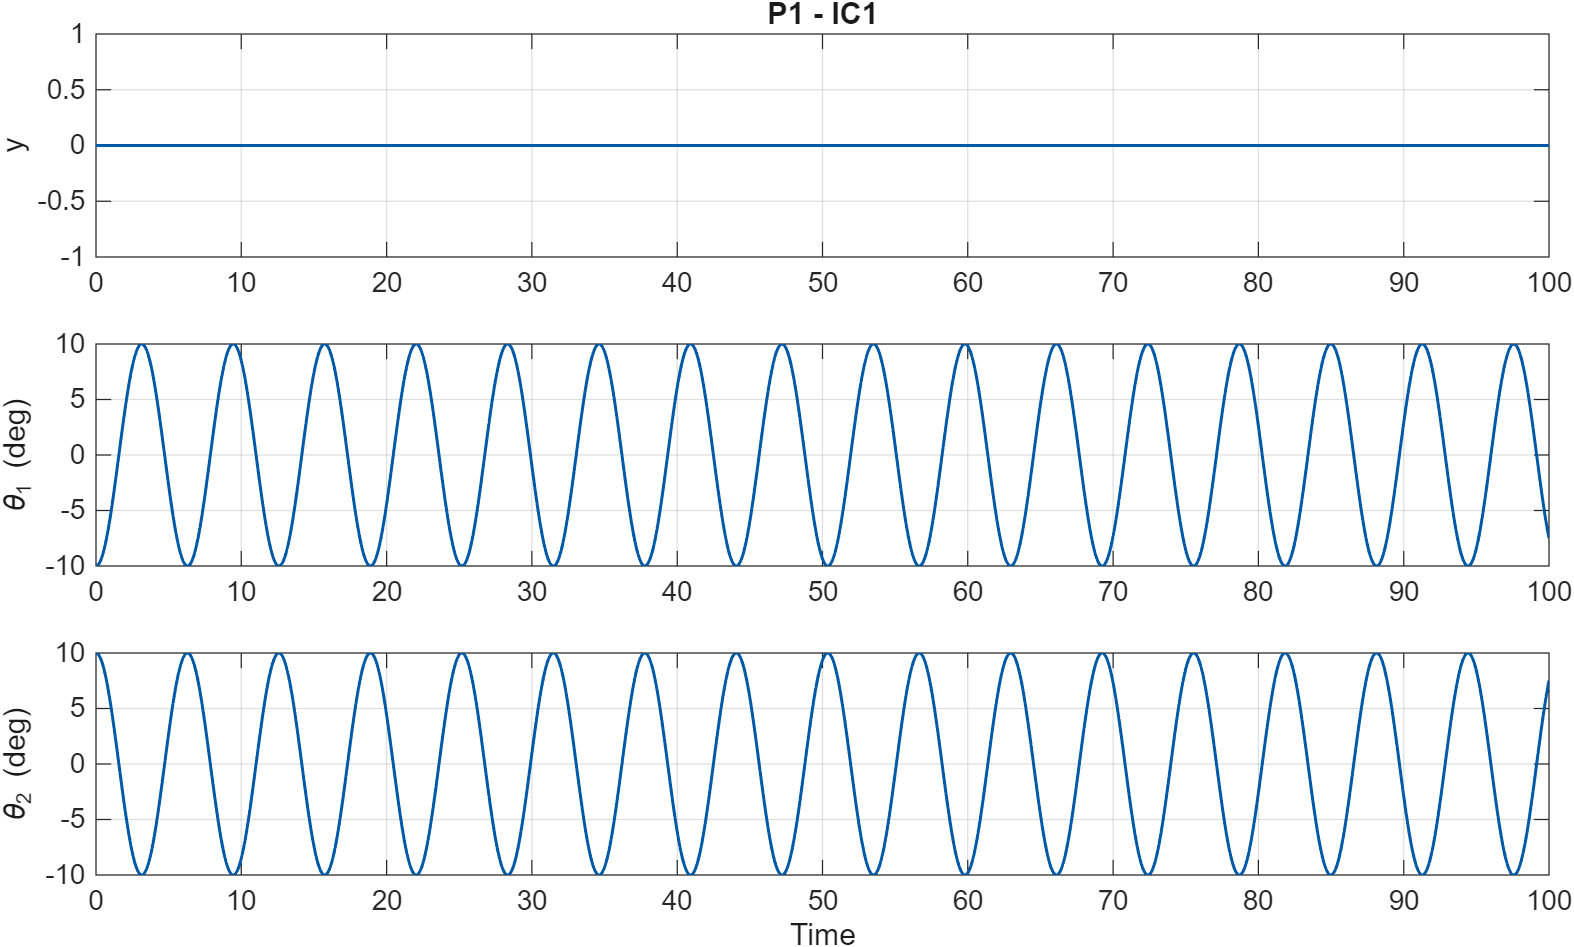
\includegraphics[width=\linewidth,height=0.35\textheight,keepaspectratio]{figures/P1_IC1.png}
\caption{P1 with IC1: cart position and pendulum angles.}
\end{figure}

\begin{figure}[!ht]
\centering
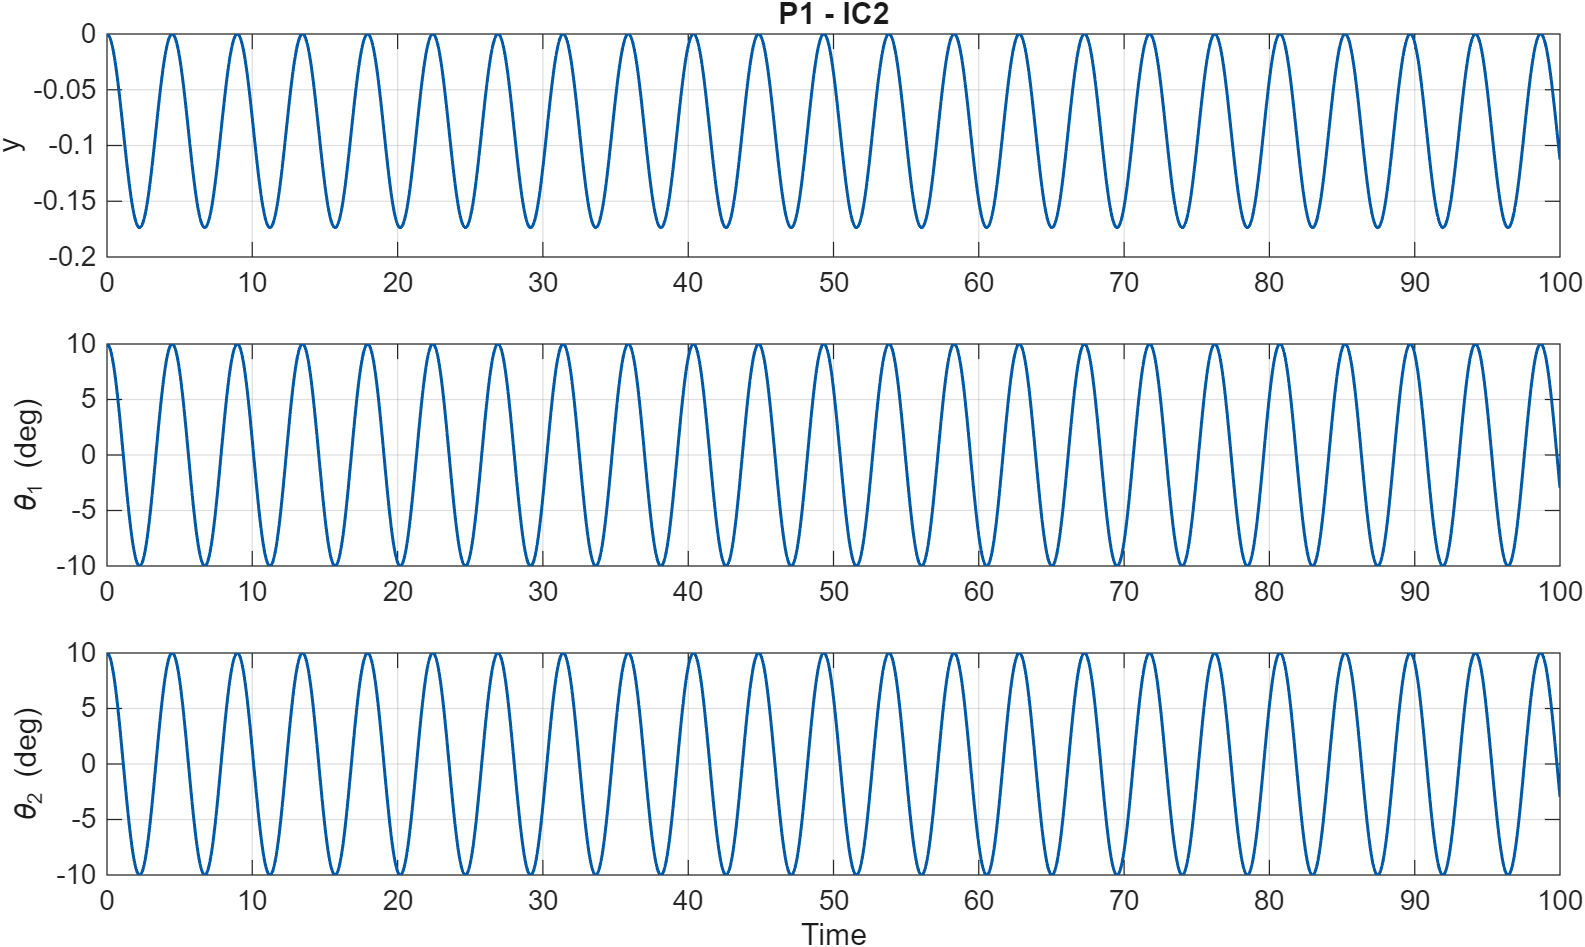
\includegraphics[width=\linewidth,height=0.35\textheight,keepaspectratio]{figures/P1_IC2.png}
\caption{P1 with IC2: cart position and pendulum angles.}
\end{figure}

\clearpage
\begin{figure}[!ht]
\centering
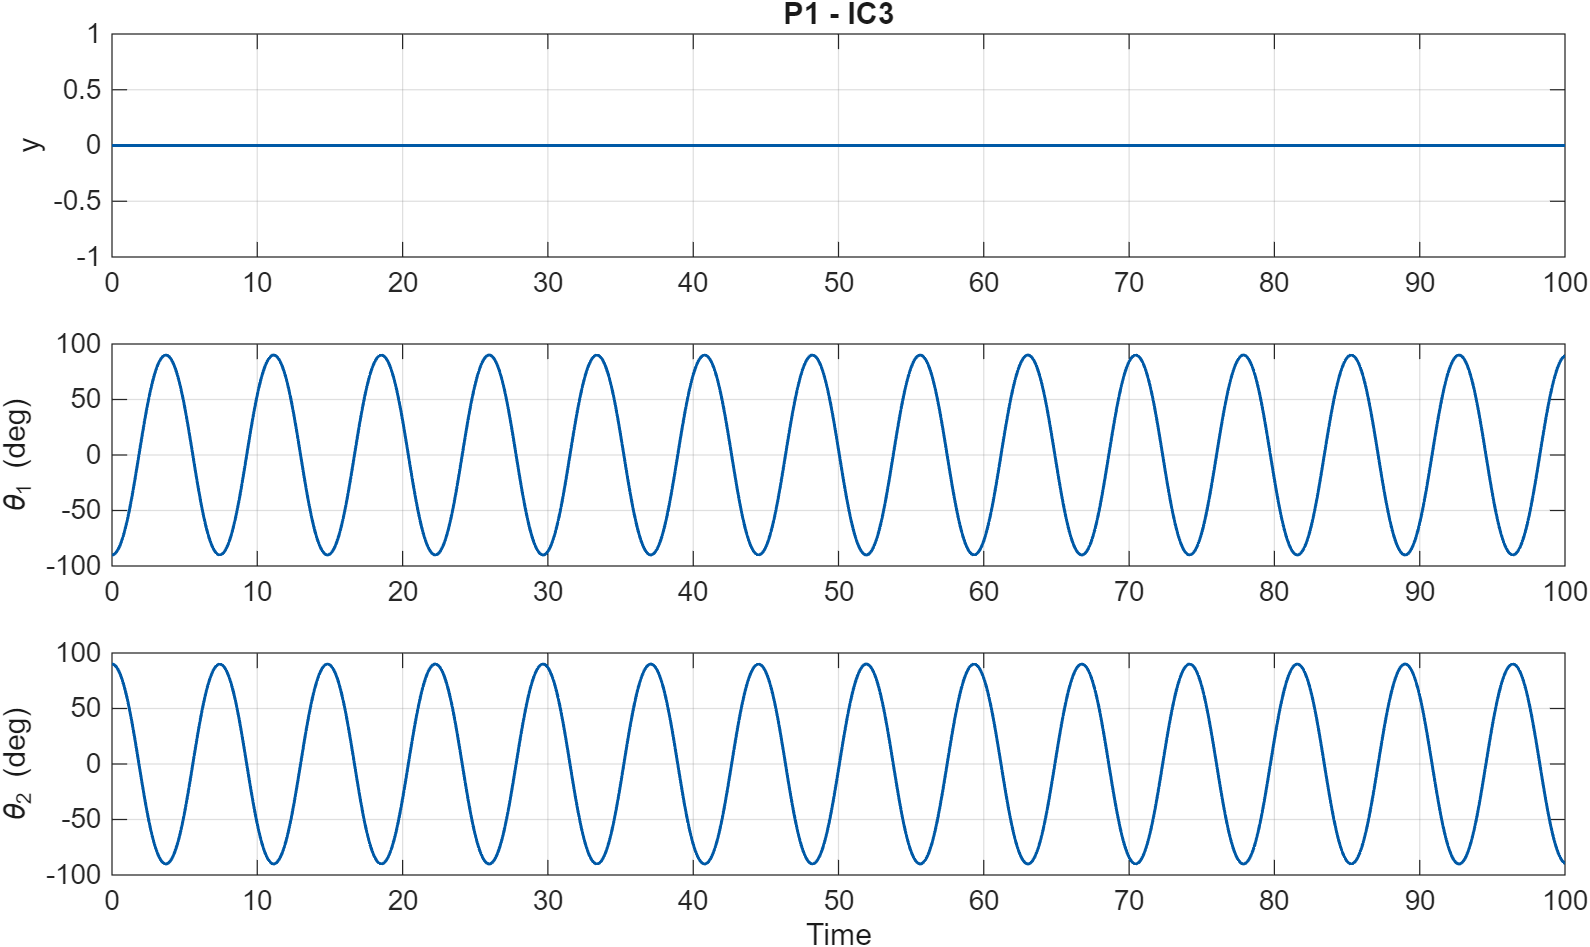
\includegraphics[width=\linewidth,height=0.35\textheight,keepaspectratio]{figures/P1_IC3.png}
\caption{P1 with IC3: cart position and pendulum angles.}
\end{figure}

\begin{figure}[!ht]
\centering
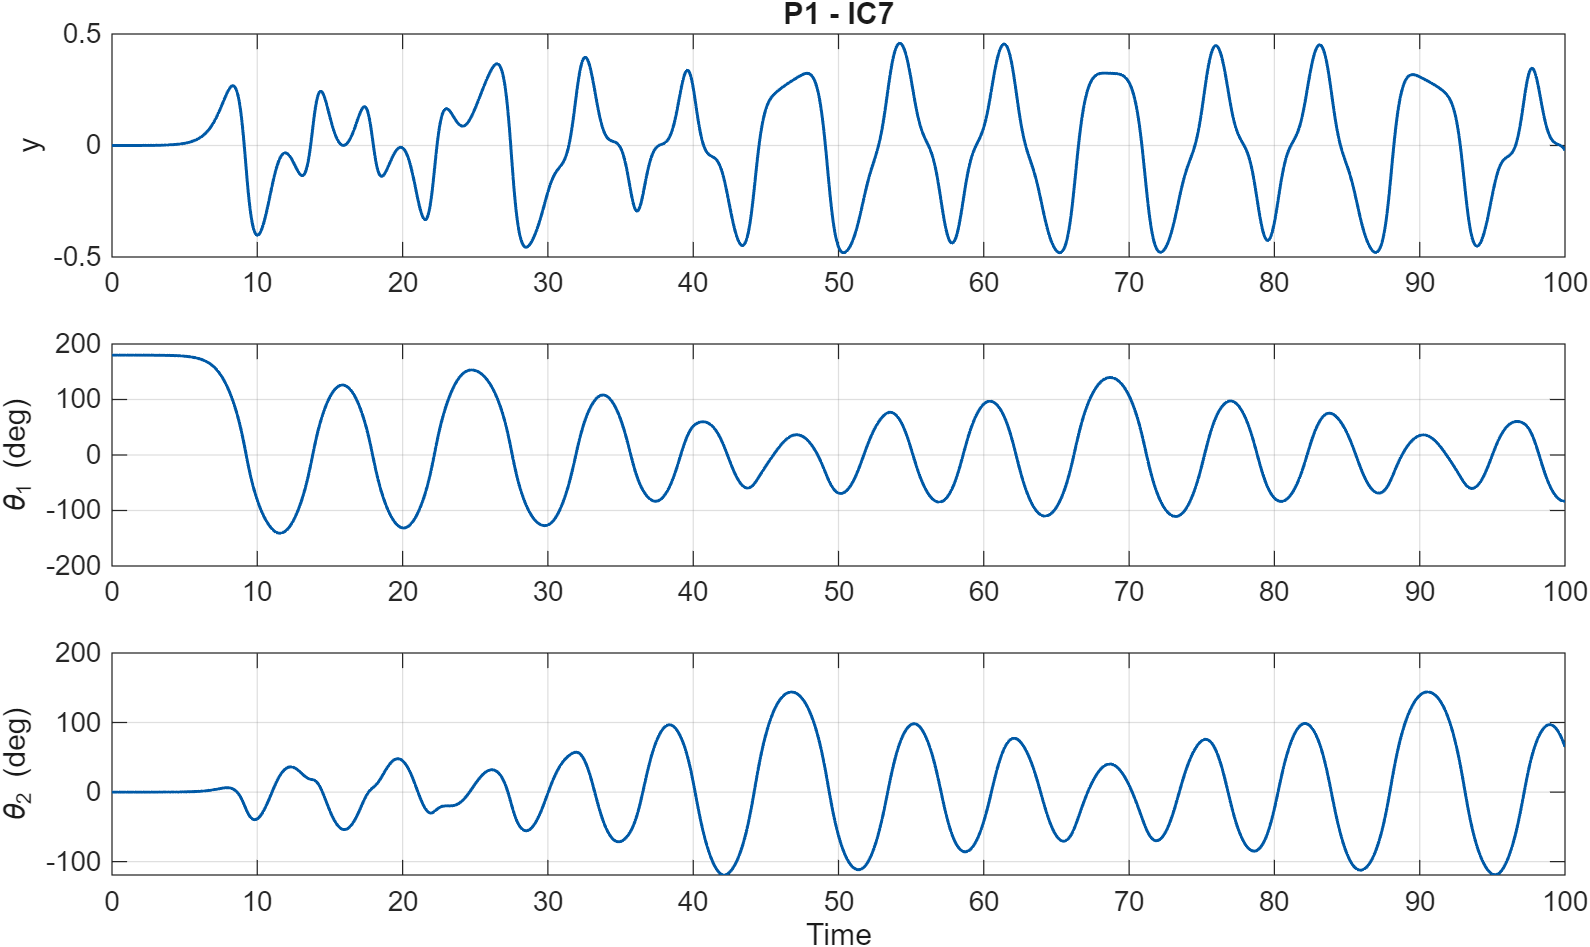
\includegraphics[width=\linewidth,height=0.35\textheight,keepaspectratio]{figures/P1_IC7.png}
\caption{P1 with IC7: cart position and pendulum angles.}
\end{figure}

\clearpage
\begin{figure}[!ht]
\centering
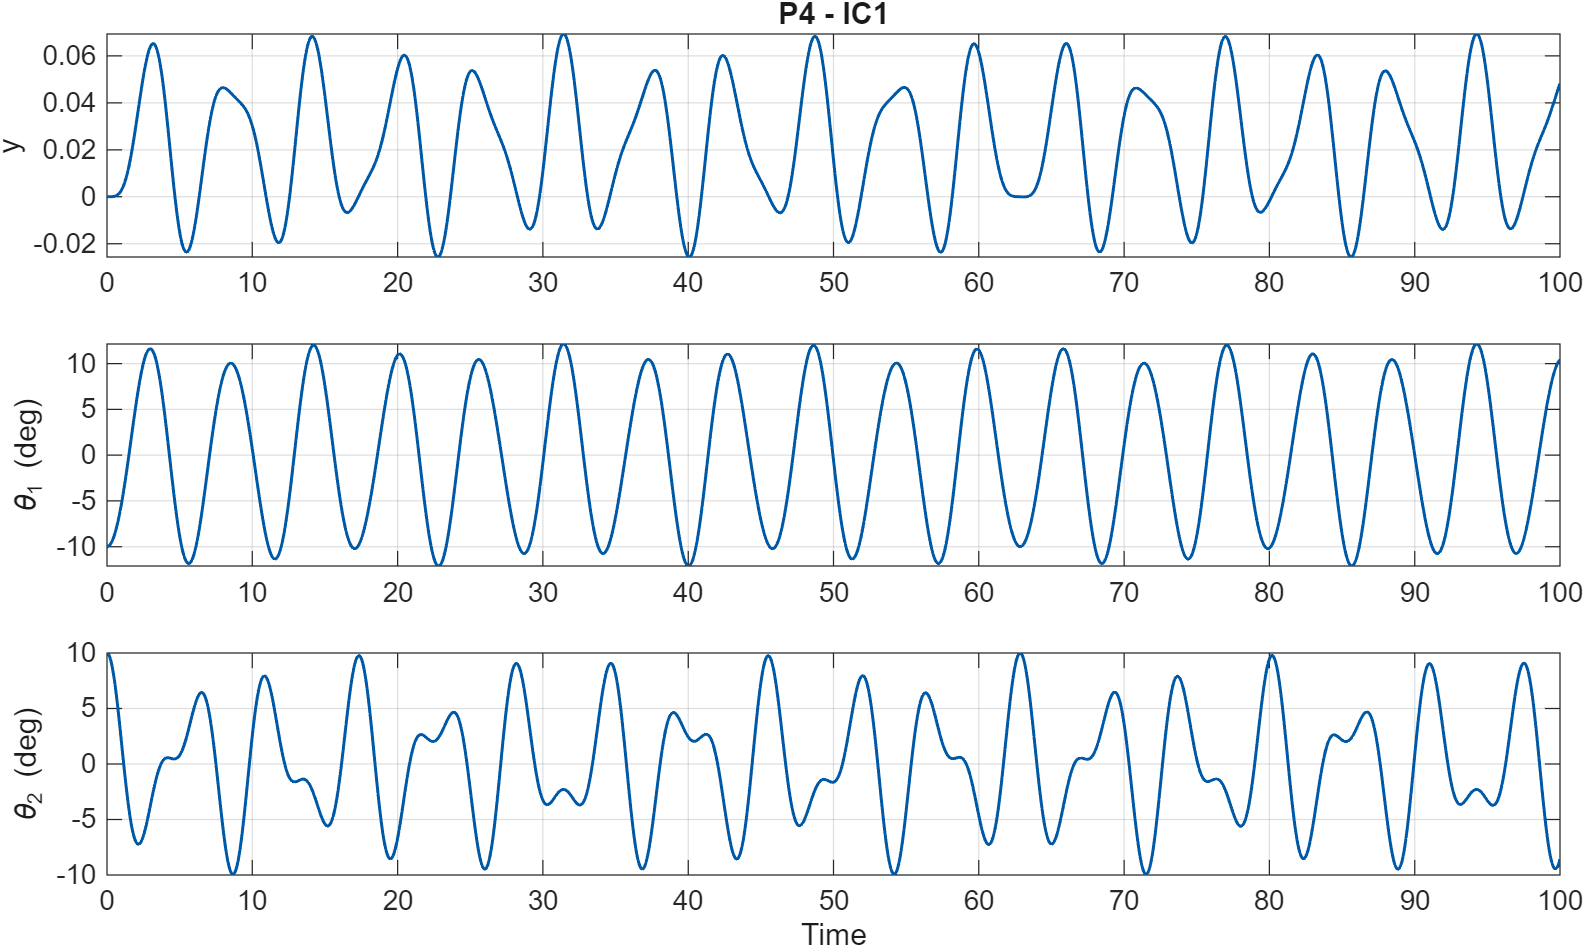
\includegraphics[width=\linewidth,height=0.35\textheight,keepaspectratio]{figures/P4_IC1.png}
\caption{P4 with IC1: cart position and pendulum angles.}
\end{figure}

\begin{figure}[!ht]
\centering
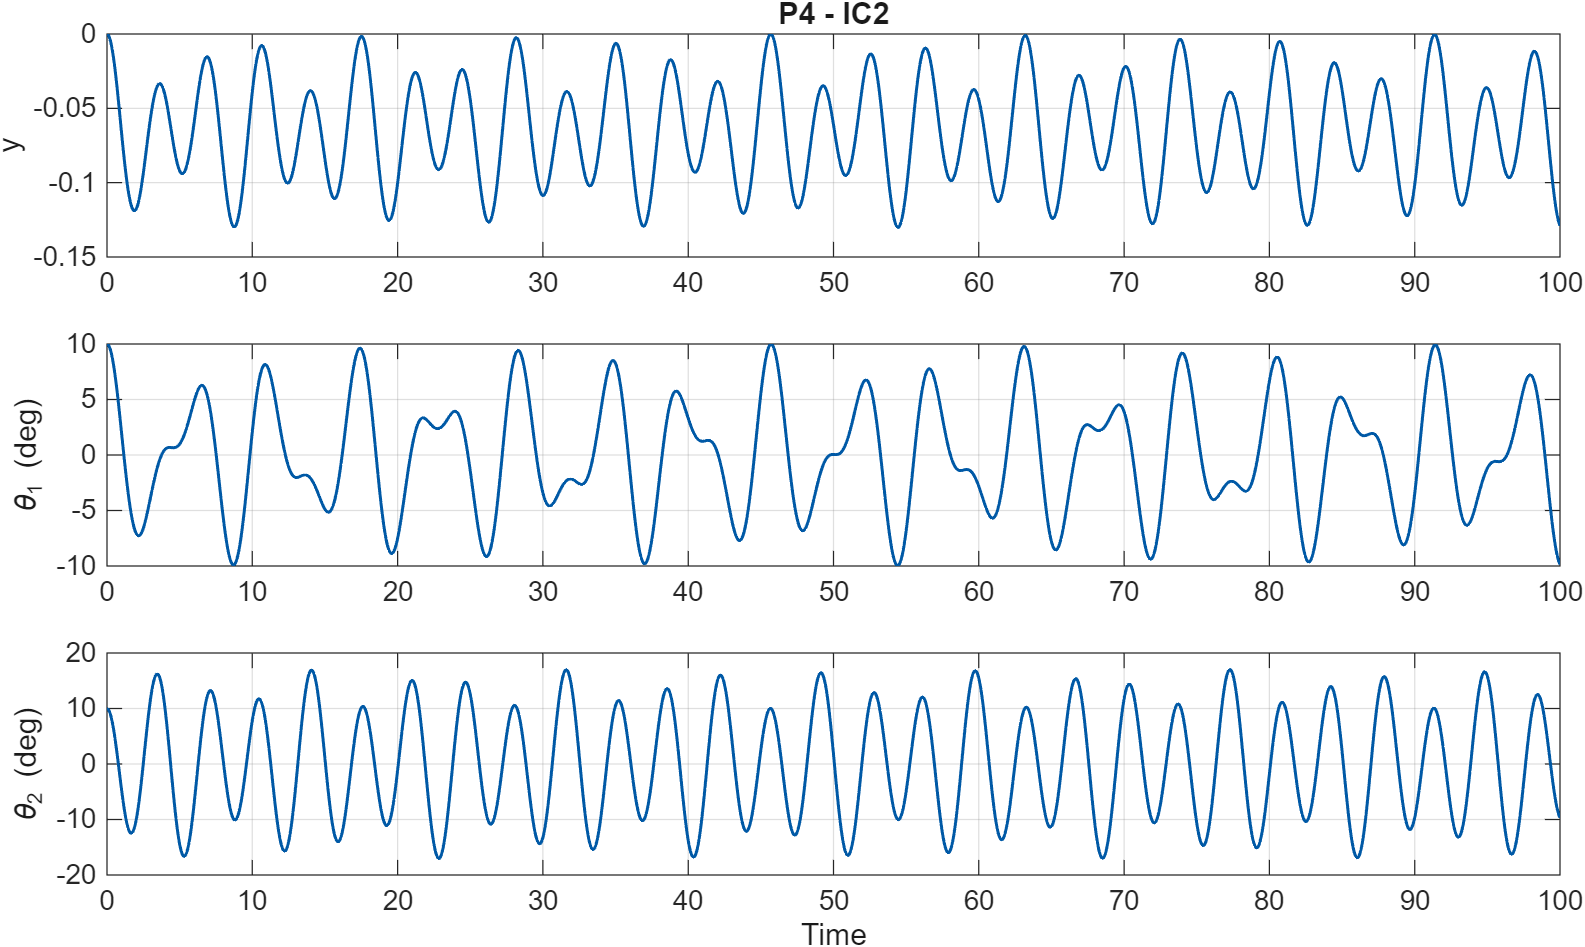
\includegraphics[width=\linewidth,height=0.35\textheight,keepaspectratio]{figures/P4_IC2.png}
\caption{P4 with IC2: cart position and pendulum angles.}
\end{figure}

\clearpage
\begin{figure}[!ht]
\centering
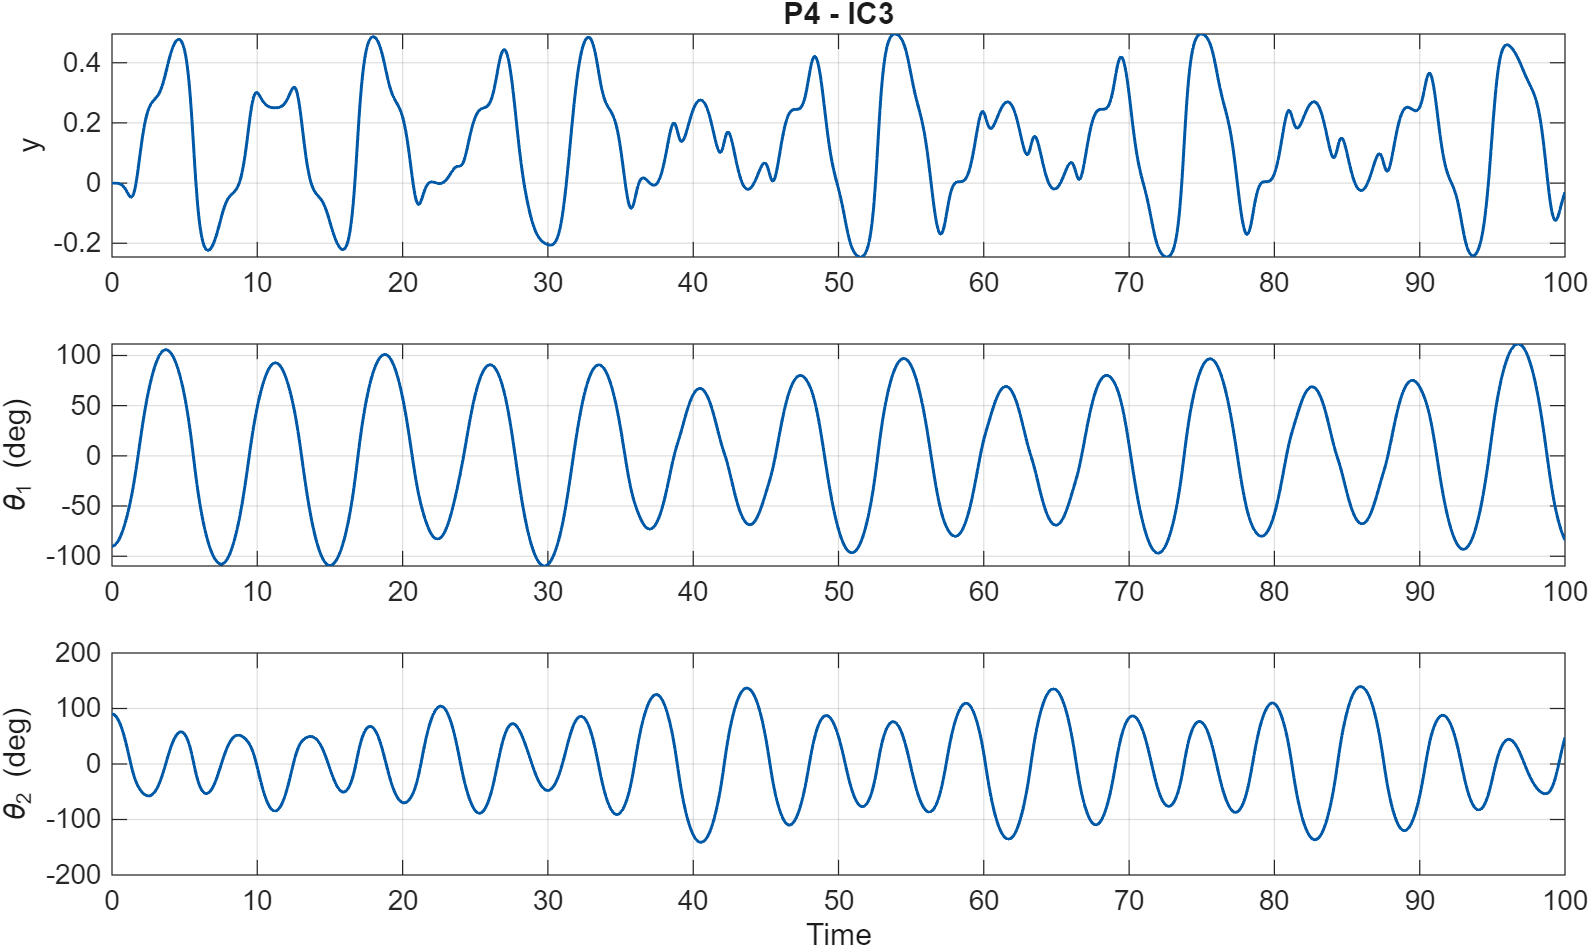
\includegraphics[width=\linewidth,height=0.35\textheight,keepaspectratio]{figures/P4_IC3.png}
\caption{P4 with IC3: cart position and pendulum angles.}
\end{figure}

\begin{figure}[!ht]
\centering
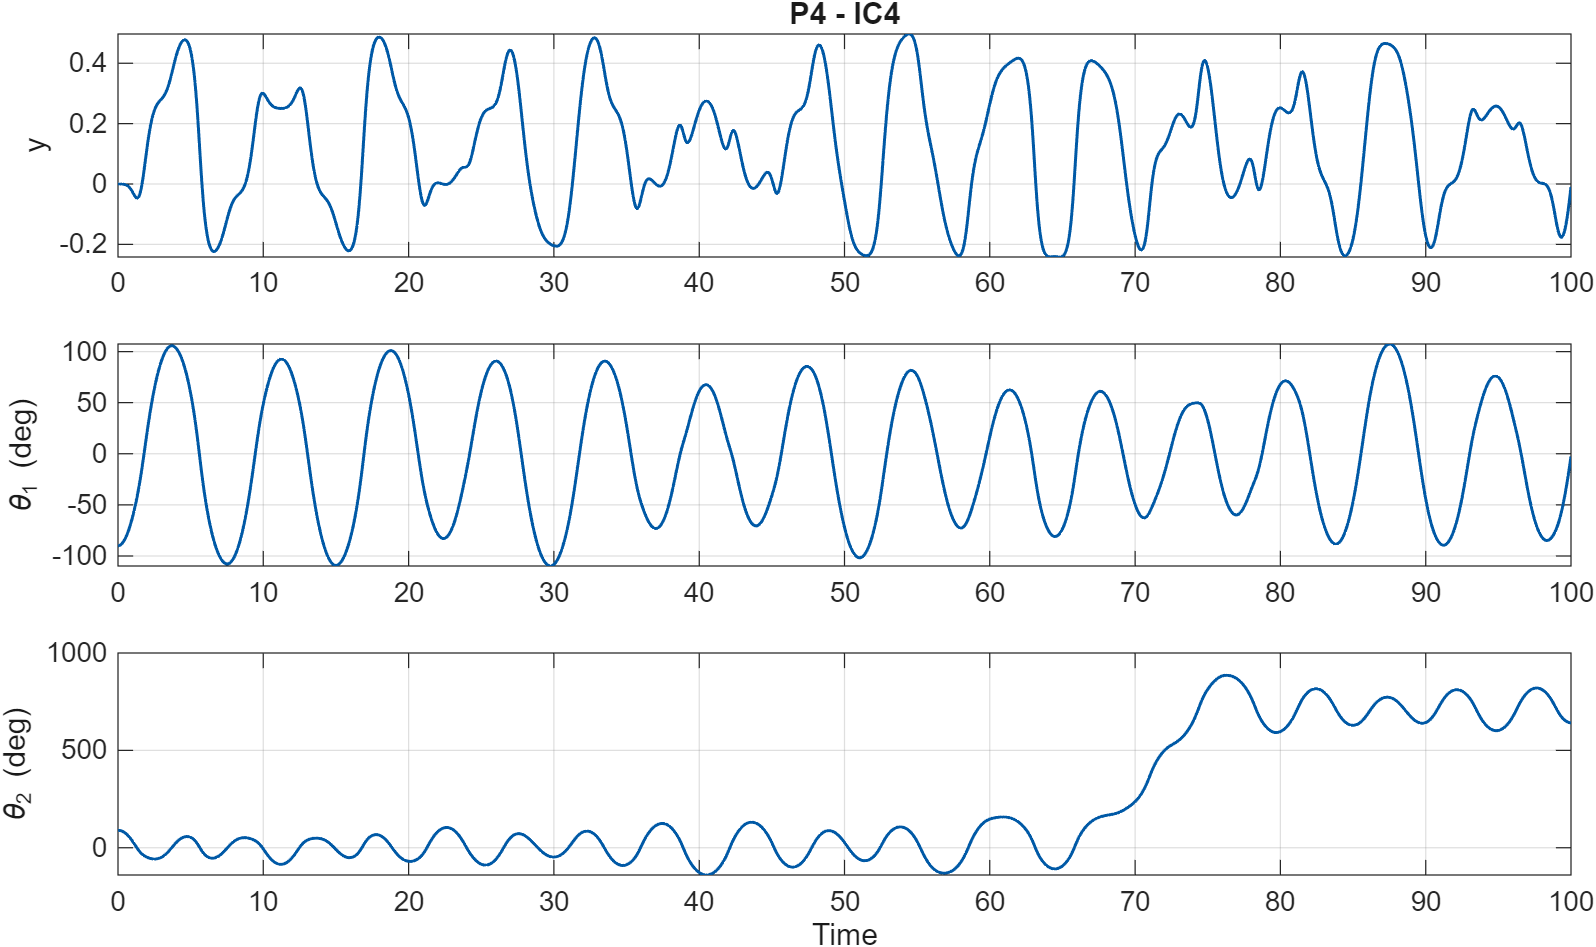
\includegraphics[width=\linewidth,height=0.35\textheight,keepaspectratio]{figures/P4_IC4.png}
\caption{P4 with IC4: cart position and pendulum angles.}
\end{figure}

\clearpage

\end{document}
